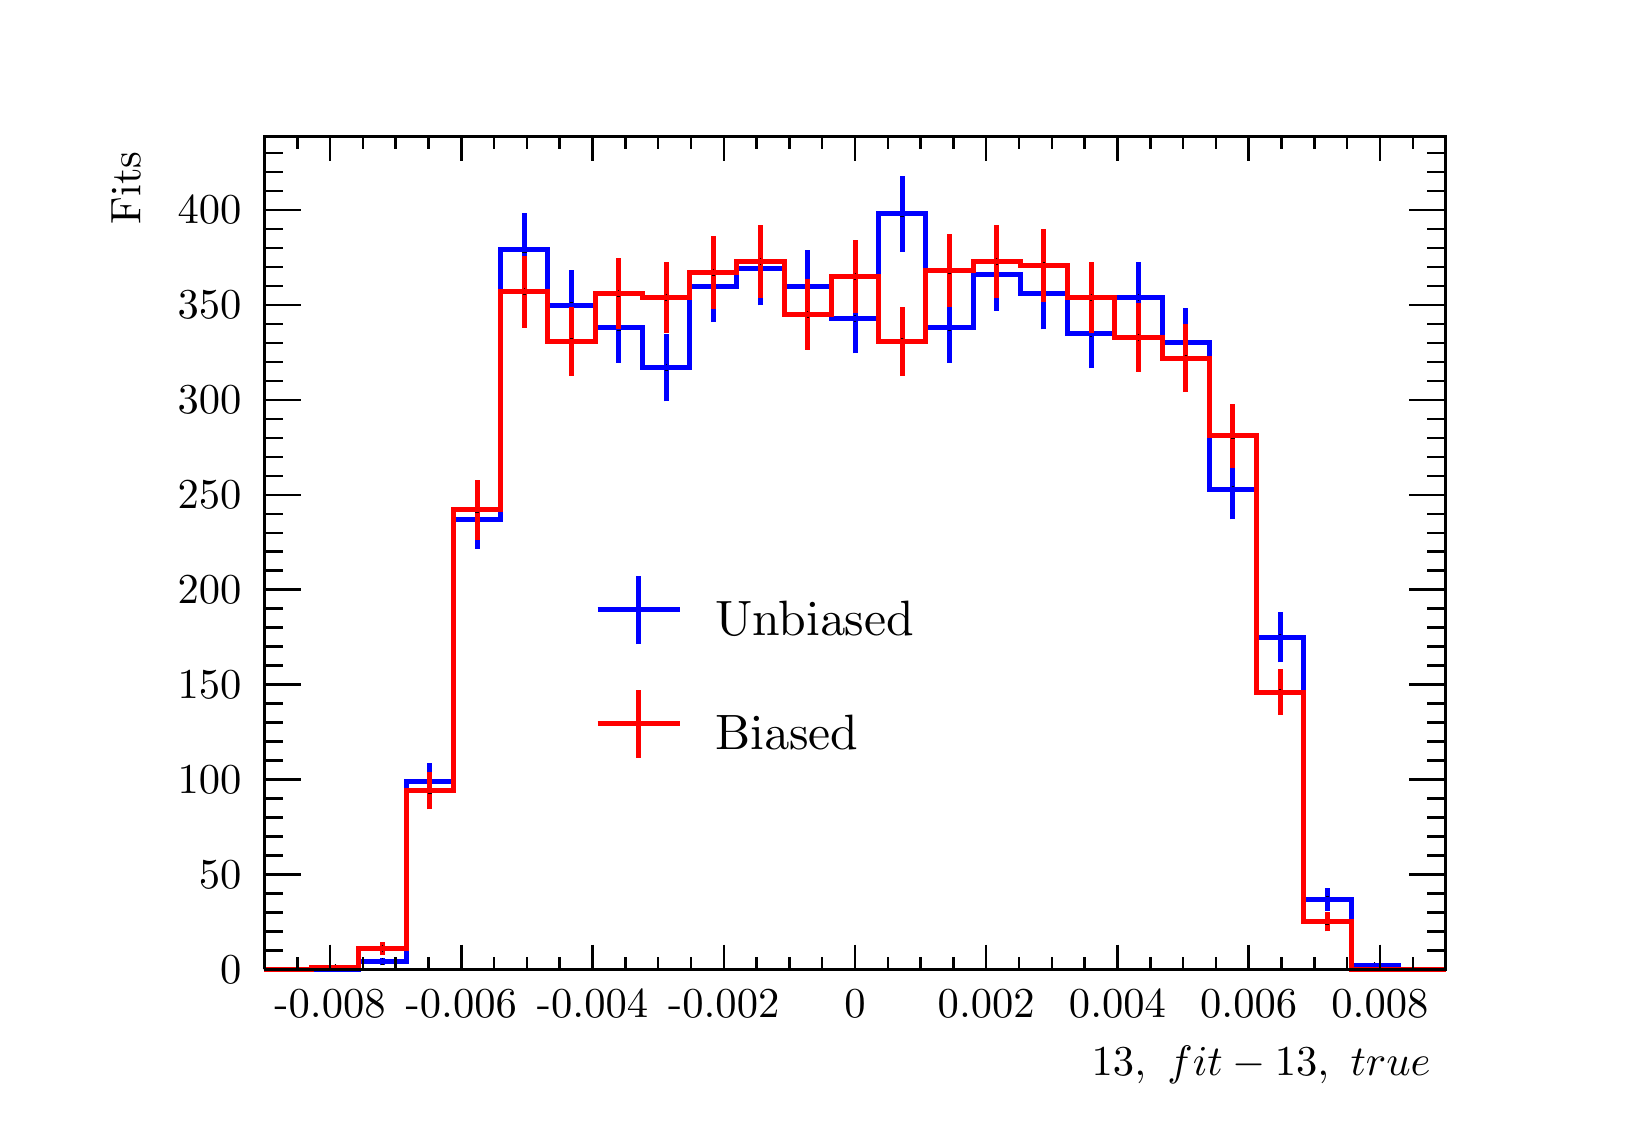
\begin{tikzpicture}
\pgfdeclareplotmark{cross} {
\pgfpathmoveto{\pgfpoint{-0.3\pgfplotmarksize}{\pgfplotmarksize}}
\pgfpathlineto{\pgfpoint{+0.3\pgfplotmarksize}{\pgfplotmarksize}}
\pgfpathlineto{\pgfpoint{+0.3\pgfplotmarksize}{0.3\pgfplotmarksize}}
\pgfpathlineto{\pgfpoint{+1\pgfplotmarksize}{0.3\pgfplotmarksize}}
\pgfpathlineto{\pgfpoint{+1\pgfplotmarksize}{-0.3\pgfplotmarksize}}
\pgfpathlineto{\pgfpoint{+0.3\pgfplotmarksize}{-0.3\pgfplotmarksize}}
\pgfpathlineto{\pgfpoint{+0.3\pgfplotmarksize}{-1.\pgfplotmarksize}}
\pgfpathlineto{\pgfpoint{-0.3\pgfplotmarksize}{-1.\pgfplotmarksize}}
\pgfpathlineto{\pgfpoint{-0.3\pgfplotmarksize}{-0.3\pgfplotmarksize}}
\pgfpathlineto{\pgfpoint{-1.\pgfplotmarksize}{-0.3\pgfplotmarksize}}
\pgfpathlineto{\pgfpoint{-1.\pgfplotmarksize}{0.3\pgfplotmarksize}}
\pgfpathlineto{\pgfpoint{-0.3\pgfplotmarksize}{0.3\pgfplotmarksize}}
\pgfpathclose
\pgfusepathqstroke
}
\pgfdeclareplotmark{cross*} {
\pgfpathmoveto{\pgfpoint{-0.3\pgfplotmarksize}{\pgfplotmarksize}}
\pgfpathlineto{\pgfpoint{+0.3\pgfplotmarksize}{\pgfplotmarksize}}
\pgfpathlineto{\pgfpoint{+0.3\pgfplotmarksize}{0.3\pgfplotmarksize}}
\pgfpathlineto{\pgfpoint{+1\pgfplotmarksize}{0.3\pgfplotmarksize}}
\pgfpathlineto{\pgfpoint{+1\pgfplotmarksize}{-0.3\pgfplotmarksize}}
\pgfpathlineto{\pgfpoint{+0.3\pgfplotmarksize}{-0.3\pgfplotmarksize}}
\pgfpathlineto{\pgfpoint{+0.3\pgfplotmarksize}{-1.\pgfplotmarksize}}
\pgfpathlineto{\pgfpoint{-0.3\pgfplotmarksize}{-1.\pgfplotmarksize}}
\pgfpathlineto{\pgfpoint{-0.3\pgfplotmarksize}{-0.3\pgfplotmarksize}}
\pgfpathlineto{\pgfpoint{-1.\pgfplotmarksize}{-0.3\pgfplotmarksize}}
\pgfpathlineto{\pgfpoint{-1.\pgfplotmarksize}{0.3\pgfplotmarksize}}
\pgfpathlineto{\pgfpoint{-0.3\pgfplotmarksize}{0.3\pgfplotmarksize}}
\pgfpathclose
\pgfusepathqfillstroke
}
\pgfdeclareplotmark{newstar} {
\pgfpathmoveto{\pgfqpoint{0pt}{\pgfplotmarksize}}
\pgfpathlineto{\pgfqpointpolar{44}{0.5\pgfplotmarksize}}
\pgfpathlineto{\pgfqpointpolar{18}{\pgfplotmarksize}}
\pgfpathlineto{\pgfqpointpolar{-20}{0.5\pgfplotmarksize}}
\pgfpathlineto{\pgfqpointpolar{-54}{\pgfplotmarksize}}
\pgfpathlineto{\pgfqpointpolar{-90}{0.5\pgfplotmarksize}}
\pgfpathlineto{\pgfqpointpolar{234}{\pgfplotmarksize}}
\pgfpathlineto{\pgfqpointpolar{198}{0.5\pgfplotmarksize}}
\pgfpathlineto{\pgfqpointpolar{162}{\pgfplotmarksize}}
\pgfpathlineto{\pgfqpointpolar{134}{0.5\pgfplotmarksize}}
\pgfpathclose
\pgfusepathqstroke
}
\pgfdeclareplotmark{newstar*} {
\pgfpathmoveto{\pgfqpoint{0pt}{\pgfplotmarksize}}
\pgfpathlineto{\pgfqpointpolar{44}{0.5\pgfplotmarksize}}
\pgfpathlineto{\pgfqpointpolar{18}{\pgfplotmarksize}}
\pgfpathlineto{\pgfqpointpolar{-20}{0.5\pgfplotmarksize}}
\pgfpathlineto{\pgfqpointpolar{-54}{\pgfplotmarksize}}
\pgfpathlineto{\pgfqpointpolar{-90}{0.5\pgfplotmarksize}}
\pgfpathlineto{\pgfqpointpolar{234}{\pgfplotmarksize}}
\pgfpathlineto{\pgfqpointpolar{198}{0.5\pgfplotmarksize}}
\pgfpathlineto{\pgfqpointpolar{162}{\pgfplotmarksize}}
\pgfpathlineto{\pgfqpointpolar{134}{0.5\pgfplotmarksize}}
\pgfpathclose
\pgfusepathqfillstroke
}
\definecolor{c}{rgb}{1,1,1};
\draw [color=c, fill=c] (0,0) rectangle (20,13.7374);
\draw [color=c, fill=c] (3,1.78586) rectangle (18,12.3636);
\definecolor{c}{rgb}{0,0,0};
\draw [c,line width=0.9] (3,1.78586) -- (3,12.3636) -- (18,12.3636) -- (18,1.78586) -- (3,1.78586);
\definecolor{c}{rgb}{1,1,1};
\draw [color=c, fill=c] (3,1.78586) rectangle (18,12.3636);
\definecolor{c}{rgb}{0,0,0};
\draw [c,line width=0.9] (3,1.78586) -- (3,12.3636) -- (18,12.3636) -- (18,1.78586) -- (3,1.78586);
\draw [c,line width=0.9] (3,1.78586) -- (3.6,1.78586) -- (3.6,1.78586) -- (4.2,1.78586) -- (4.2,1.78586) -- (4.8,1.78586) -- (4.8,1.78586) -- (5.4,1.78586) -- (5.4,1.78586) -- (6,1.78586) -- (6,1.78586) -- (6.6,1.78586) -- (6.6,1.78586) --
 (7.2,1.78586) -- (7.2,1.78586) -- (7.8,1.78586) -- (7.8,1.78586) -- (8.4,1.78586) -- (8.4,1.78586) -- (9,1.78586) -- (9,1.78586) -- (9.6,1.78586) -- (9.6,1.78586) -- (10.2,1.78586) -- (10.2,1.78586) -- (10.8,1.78586) -- (10.8,1.78586) --
 (11.4,1.78586) -- (11.4,1.78586) -- (12,1.78586) -- (12,1.78586) -- (12.6,1.78586) -- (12.6,1.78586) -- (13.2,1.78586) -- (13.2,1.78586) -- (13.8,1.78586) -- (13.8,1.78586) -- (14.4,1.78586) -- (14.4,1.78586) -- (15,1.78586) -- (15,1.78586) --
 (15.6,1.78586) -- (15.6,1.78586) -- (16.2,1.78586) -- (16.2,1.78586) -- (16.8,1.78586) -- (16.8,1.78586) -- (17.4,1.78586) -- (17.4,1.78586) -- (18,1.78586) -- (18,1.78586);
\draw [c,line width=0.9] (3,1.78586) -- (18,1.78586);
\draw [c,line width=0.9] (3.83333,2.09495) -- (3.83333,1.78586);
\draw [c,line width=0.9] (4.25,1.9404) -- (4.25,1.78586);
\draw [c,line width=0.9] (4.66667,1.9404) -- (4.66667,1.78586);
\draw [c,line width=0.9] (5.08333,1.9404) -- (5.08333,1.78586);
\draw [c,line width=0.9] (5.5,2.09495) -- (5.5,1.78586);
\draw [c,line width=0.9] (5.91667,1.9404) -- (5.91667,1.78586);
\draw [c,line width=0.9] (6.33333,1.9404) -- (6.33333,1.78586);
\draw [c,line width=0.9] (6.75,1.9404) -- (6.75,1.78586);
\draw [c,line width=0.9] (7.16667,2.09495) -- (7.16667,1.78586);
\draw [c,line width=0.9] (7.58333,1.9404) -- (7.58333,1.78586);
\draw [c,line width=0.9] (8,1.9404) -- (8,1.78586);
\draw [c,line width=0.9] (8.41667,1.9404) -- (8.41667,1.78586);
\draw [c,line width=0.9] (8.83333,2.09495) -- (8.83333,1.78586);
\draw [c,line width=0.9] (9.25,1.9404) -- (9.25,1.78586);
\draw [c,line width=0.9] (9.66667,1.9404) -- (9.66667,1.78586);
\draw [c,line width=0.9] (10.0833,1.9404) -- (10.0833,1.78586);
\draw [c,line width=0.9] (10.5,2.09495) -- (10.5,1.78586);
\draw [c,line width=0.9] (10.9167,1.9404) -- (10.9167,1.78586);
\draw [c,line width=0.9] (11.3333,1.9404) -- (11.3333,1.78586);
\draw [c,line width=0.9] (11.75,1.9404) -- (11.75,1.78586);
\draw [c,line width=0.9] (12.1667,2.09495) -- (12.1667,1.78586);
\draw [c,line width=0.9] (12.5833,1.9404) -- (12.5833,1.78586);
\draw [c,line width=0.9] (13,1.9404) -- (13,1.78586);
\draw [c,line width=0.9] (13.4167,1.9404) -- (13.4167,1.78586);
\draw [c,line width=0.9] (13.8333,2.09495) -- (13.8333,1.78586);
\draw [c,line width=0.9] (14.25,1.9404) -- (14.25,1.78586);
\draw [c,line width=0.9] (14.6667,1.9404) -- (14.6667,1.78586);
\draw [c,line width=0.9] (15.0833,1.9404) -- (15.0833,1.78586);
\draw [c,line width=0.9] (15.5,2.09495) -- (15.5,1.78586);
\draw [c,line width=0.9] (15.9167,1.9404) -- (15.9167,1.78586);
\draw [c,line width=0.9] (16.3333,1.9404) -- (16.3333,1.78586);
\draw [c,line width=0.9] (16.75,1.9404) -- (16.75,1.78586);
\draw [c,line width=0.9] (17.1667,2.09495) -- (17.1667,1.78586);
\draw [c,line width=0.9] (3.83333,2.09495) -- (3.83333,1.78586);
\draw [c,line width=0.9] (3.41667,1.9404) -- (3.41667,1.78586);
\draw [c,line width=0.9] (17.1667,2.09495) -- (17.1667,1.78586);
\draw [c,line width=0.9] (17.5833,1.9404) -- (17.5833,1.78586);
\draw [anchor=base] (3.83333,1.16768) node[scale=1.53833, color=c, rotate=0]{-0.008};
\draw [anchor=base] (5.5,1.16768) node[scale=1.53833, color=c, rotate=0]{-0.006};
\draw [anchor=base] (7.16667,1.16768) node[scale=1.53833, color=c, rotate=0]{-0.004};
\draw [anchor=base] (8.83333,1.16768) node[scale=1.53833, color=c, rotate=0]{-0.002};
\draw [anchor=base] (10.5,1.16768) node[scale=1.53833, color=c, rotate=0]{0};
\draw [anchor=base] (12.1667,1.16768) node[scale=1.53833, color=c, rotate=0]{0.002};
\draw [anchor=base] (13.8333,1.16768) node[scale=1.53833, color=c, rotate=0]{0.004};
\draw [anchor=base] (15.5,1.16768) node[scale=1.53833, color=c, rotate=0]{0.006};
\draw [anchor=base] (17.1667,1.16768) node[scale=1.53833, color=c, rotate=0]{0.008};
\draw [anchor= east] (18,0.57697) node[scale=1.53833, color=c, rotate=0]{$\thetai{13,~\text{fit}} - \thetai{13,~\text{true}}$};
\draw [c,line width=0.9] (3,12.3636) -- (18,12.3636);
\draw [c,line width=0.9] (3.83333,12.0545) -- (3.83333,12.3636);
\draw [c,line width=0.9] (4.25,12.2091) -- (4.25,12.3636);
\draw [c,line width=0.9] (4.66667,12.2091) -- (4.66667,12.3636);
\draw [c,line width=0.9] (5.08333,12.2091) -- (5.08333,12.3636);
\draw [c,line width=0.9] (5.5,12.0545) -- (5.5,12.3636);
\draw [c,line width=0.9] (5.91667,12.2091) -- (5.91667,12.3636);
\draw [c,line width=0.9] (6.33333,12.2091) -- (6.33333,12.3636);
\draw [c,line width=0.9] (6.75,12.2091) -- (6.75,12.3636);
\draw [c,line width=0.9] (7.16667,12.0545) -- (7.16667,12.3636);
\draw [c,line width=0.9] (7.58333,12.2091) -- (7.58333,12.3636);
\draw [c,line width=0.9] (8,12.2091) -- (8,12.3636);
\draw [c,line width=0.9] (8.41667,12.2091) -- (8.41667,12.3636);
\draw [c,line width=0.9] (8.83333,12.0545) -- (8.83333,12.3636);
\draw [c,line width=0.9] (9.25,12.2091) -- (9.25,12.3636);
\draw [c,line width=0.9] (9.66667,12.2091) -- (9.66667,12.3636);
\draw [c,line width=0.9] (10.0833,12.2091) -- (10.0833,12.3636);
\draw [c,line width=0.9] (10.5,12.0545) -- (10.5,12.3636);
\draw [c,line width=0.9] (10.9167,12.2091) -- (10.9167,12.3636);
\draw [c,line width=0.9] (11.3333,12.2091) -- (11.3333,12.3636);
\draw [c,line width=0.9] (11.75,12.2091) -- (11.75,12.3636);
\draw [c,line width=0.9] (12.1667,12.0545) -- (12.1667,12.3636);
\draw [c,line width=0.9] (12.5833,12.2091) -- (12.5833,12.3636);
\draw [c,line width=0.9] (13,12.2091) -- (13,12.3636);
\draw [c,line width=0.9] (13.4167,12.2091) -- (13.4167,12.3636);
\draw [c,line width=0.9] (13.8333,12.0545) -- (13.8333,12.3636);
\draw [c,line width=0.9] (14.25,12.2091) -- (14.25,12.3636);
\draw [c,line width=0.9] (14.6667,12.2091) -- (14.6667,12.3636);
\draw [c,line width=0.9] (15.0833,12.2091) -- (15.0833,12.3636);
\draw [c,line width=0.9] (15.5,12.0545) -- (15.5,12.3636);
\draw [c,line width=0.9] (15.9167,12.2091) -- (15.9167,12.3636);
\draw [c,line width=0.9] (16.3333,12.2091) -- (16.3333,12.3636);
\draw [c,line width=0.9] (16.75,12.2091) -- (16.75,12.3636);
\draw [c,line width=0.9] (17.1667,12.0545) -- (17.1667,12.3636);
\draw [c,line width=0.9] (3.83333,12.0545) -- (3.83333,12.3636);
\draw [c,line width=0.9] (3.41667,12.2091) -- (3.41667,12.3636);
\draw [c,line width=0.9] (17.1667,12.0545) -- (17.1667,12.3636);
\draw [c,line width=0.9] (17.5833,12.2091) -- (17.5833,12.3636);
\draw [c,line width=0.9] (3,1.78586) -- (3,12.3636);
\draw [c,line width=0.9] (3.462,1.78586) -- (3,1.78586);
\draw [c,line width=0.9] (3.231,2.02689) -- (3,2.02689);
\draw [c,line width=0.9] (3.231,2.26793) -- (3,2.26793);
\draw [c,line width=0.9] (3.231,2.50896) -- (3,2.50896);
\draw [c,line width=0.9] (3.231,2.75) -- (3,2.75);
\draw [c,line width=0.9] (3.462,2.99104) -- (3,2.99104);
\draw [c,line width=0.9] (3.231,3.23207) -- (3,3.23207);
\draw [c,line width=0.9] (3.231,3.47311) -- (3,3.47311);
\draw [c,line width=0.9] (3.231,3.71414) -- (3,3.71414);
\draw [c,line width=0.9] (3.231,3.95518) -- (3,3.95518);
\draw [c,line width=0.9] (3.462,4.19621) -- (3,4.19621);
\draw [c,line width=0.9] (3.231,4.43725) -- (3,4.43725);
\draw [c,line width=0.9] (3.231,4.67828) -- (3,4.67828);
\draw [c,line width=0.9] (3.231,4.91932) -- (3,4.91932);
\draw [c,line width=0.9] (3.231,5.16035) -- (3,5.16035);
\draw [c,line width=0.9] (3.462,5.40139) -- (3,5.40139);
\draw [c,line width=0.9] (3.231,5.64243) -- (3,5.64243);
\draw [c,line width=0.9] (3.231,5.88346) -- (3,5.88346);
\draw [c,line width=0.9] (3.231,6.1245) -- (3,6.1245);
\draw [c,line width=0.9] (3.231,6.36553) -- (3,6.36553);
\draw [c,line width=0.9] (3.462,6.60657) -- (3,6.60657);
\draw [c,line width=0.9] (3.231,6.8476) -- (3,6.8476);
\draw [c,line width=0.9] (3.231,7.08864) -- (3,7.08864);
\draw [c,line width=0.9] (3.231,7.32967) -- (3,7.32967);
\draw [c,line width=0.9] (3.231,7.57071) -- (3,7.57071);
\draw [c,line width=0.9] (3.462,7.81174) -- (3,7.81174);
\draw [c,line width=0.9] (3.231,8.05278) -- (3,8.05278);
\draw [c,line width=0.9] (3.231,8.29381) -- (3,8.29381);
\draw [c,line width=0.9] (3.231,8.53485) -- (3,8.53485);
\draw [c,line width=0.9] (3.231,8.77589) -- (3,8.77589);
\draw [c,line width=0.9] (3.462,9.01692) -- (3,9.01692);
\draw [c,line width=0.9] (3.231,9.25796) -- (3,9.25796);
\draw [c,line width=0.9] (3.231,9.49899) -- (3,9.49899);
\draw [c,line width=0.9] (3.231,9.74003) -- (3,9.74003);
\draw [c,line width=0.9] (3.231,9.98106) -- (3,9.98106);
\draw [c,line width=0.9] (3.462,10.2221) -- (3,10.2221);
\draw [c,line width=0.9] (3.231,10.4631) -- (3,10.4631);
\draw [c,line width=0.9] (3.231,10.7042) -- (3,10.7042);
\draw [c,line width=0.9] (3.231,10.9452) -- (3,10.9452);
\draw [c,line width=0.9] (3.231,11.1862) -- (3,11.1862);
\draw [c,line width=0.9] (3.462,11.4273) -- (3,11.4273);
\draw [c,line width=0.9] (3.462,11.4273) -- (3,11.4273);
\draw [c,line width=0.9] (3.231,11.6683) -- (3,11.6683);
\draw [c,line width=0.9] (3.231,11.9093) -- (3,11.9093);
\draw [c,line width=0.9] (3.231,12.1504) -- (3,12.1504);
\draw [anchor= east] (2.9,1.78586) node[scale=1.53833, color=c, rotate=0]{0};
\draw [anchor= east] (2.9,2.99104) node[scale=1.53833, color=c, rotate=0]{50};
\draw [anchor= east] (2.9,4.19621) node[scale=1.53833, color=c, rotate=0]{100};
\draw [anchor= east] (2.9,5.40139) node[scale=1.53833, color=c, rotate=0]{150};
\draw [anchor= east] (2.9,6.60657) node[scale=1.53833, color=c, rotate=0]{200};
\draw [anchor= east] (2.9,7.81174) node[scale=1.53833, color=c, rotate=0]{250};
\draw [anchor= east] (2.9,9.01692) node[scale=1.53833, color=c, rotate=0]{300};
\draw [anchor= east] (2.9,10.2221) node[scale=1.53833, color=c, rotate=0]{350};
\draw [anchor= east] (2.9,11.4273) node[scale=1.53833, color=c, rotate=0]{400};
\draw [anchor= east] (1.24,12.3636) node[scale=1.53833, color=c, rotate=90]{ Fits};
\draw [c,line width=0.9] (18,1.78586) -- (18,12.3636);
\draw [c,line width=0.9] (17.538,1.78586) -- (18,1.78586);
\draw [c,line width=0.9] (17.769,2.02689) -- (18,2.02689);
\draw [c,line width=0.9] (17.769,2.26793) -- (18,2.26793);
\draw [c,line width=0.9] (17.769,2.50896) -- (18,2.50896);
\draw [c,line width=0.9] (17.769,2.75) -- (18,2.75);
\draw [c,line width=0.9] (17.538,2.99104) -- (18,2.99104);
\draw [c,line width=0.9] (17.769,3.23207) -- (18,3.23207);
\draw [c,line width=0.9] (17.769,3.47311) -- (18,3.47311);
\draw [c,line width=0.9] (17.769,3.71414) -- (18,3.71414);
\draw [c,line width=0.9] (17.769,3.95518) -- (18,3.95518);
\draw [c,line width=0.9] (17.538,4.19621) -- (18,4.19621);
\draw [c,line width=0.9] (17.769,4.43725) -- (18,4.43725);
\draw [c,line width=0.9] (17.769,4.67828) -- (18,4.67828);
\draw [c,line width=0.9] (17.769,4.91932) -- (18,4.91932);
\draw [c,line width=0.9] (17.769,5.16035) -- (18,5.16035);
\draw [c,line width=0.9] (17.538,5.40139) -- (18,5.40139);
\draw [c,line width=0.9] (17.769,5.64243) -- (18,5.64243);
\draw [c,line width=0.9] (17.769,5.88346) -- (18,5.88346);
\draw [c,line width=0.9] (17.769,6.1245) -- (18,6.1245);
\draw [c,line width=0.9] (17.769,6.36553) -- (18,6.36553);
\draw [c,line width=0.9] (17.538,6.60657) -- (18,6.60657);
\draw [c,line width=0.9] (17.769,6.8476) -- (18,6.8476);
\draw [c,line width=0.9] (17.769,7.08864) -- (18,7.08864);
\draw [c,line width=0.9] (17.769,7.32967) -- (18,7.32967);
\draw [c,line width=0.9] (17.769,7.57071) -- (18,7.57071);
\draw [c,line width=0.9] (17.538,7.81174) -- (18,7.81174);
\draw [c,line width=0.9] (17.769,8.05278) -- (18,8.05278);
\draw [c,line width=0.9] (17.769,8.29381) -- (18,8.29381);
\draw [c,line width=0.9] (17.769,8.53485) -- (18,8.53485);
\draw [c,line width=0.9] (17.769,8.77589) -- (18,8.77589);
\draw [c,line width=0.9] (17.538,9.01692) -- (18,9.01692);
\draw [c,line width=0.9] (17.769,9.25796) -- (18,9.25796);
\draw [c,line width=0.9] (17.769,9.49899) -- (18,9.49899);
\draw [c,line width=0.9] (17.769,9.74003) -- (18,9.74003);
\draw [c,line width=0.9] (17.769,9.98106) -- (18,9.98106);
\draw [c,line width=0.9] (17.538,10.2221) -- (18,10.2221);
\draw [c,line width=0.9] (17.769,10.4631) -- (18,10.4631);
\draw [c,line width=0.9] (17.769,10.7042) -- (18,10.7042);
\draw [c,line width=0.9] (17.769,10.9452) -- (18,10.9452);
\draw [c,line width=0.9] (17.769,11.1862) -- (18,11.1862);
\draw [c,line width=0.9] (17.538,11.4273) -- (18,11.4273);
\draw [c,line width=0.9] (17.538,11.4273) -- (18,11.4273);
\draw [c,line width=0.9] (17.769,11.6683) -- (18,11.6683);
\draw [c,line width=0.9] (17.769,11.9093) -- (18,11.9093);
\draw [c,line width=0.9] (17.769,12.1504) -- (18,12.1504);
\definecolor{c}{rgb}{0,0,1};
\draw [c,line width=1.8] (4.5,1.83407) -- (4.5,1.88227);
\draw [c,line width=1.8] (4.5,1.88227) -- (4.5,1.93048);
\definecolor{c}{rgb}{0,0,0};
\foreach \P in {(4.5,1.88227)}{\draw[mark options={color=c,fill=c},mark size=2.402402pt, line width=0.000000pt, mark=*,mark size=1pt] plot coordinates {\P};}
\definecolor{c}{rgb}{0,0,1};
\draw [c,line width=1.8] (5.1,3.93228) -- (5.1,4.17211);
\draw [c,line width=1.8] (5.1,4.17211) -- (5.1,4.41194);
\definecolor{c}{rgb}{0,0,0};
\foreach \P in {(5.1,4.17211)}{\draw[mark options={color=c,fill=c},mark size=2.402402pt, line width=0.000000pt, mark=*,mark size=1pt] plot coordinates {\P};}
\definecolor{c}{rgb}{0,0,1};
\draw [c,line width=1.8] (5.7,7.12733) -- (5.7,7.4984);
\draw [c,line width=1.8] (5.7,7.4984) -- (5.7,7.86947);
\definecolor{c}{rgb}{0,0,0};
\foreach \P in {(5.7,7.4984)}{\draw[mark options={color=c,fill=c},mark size=2.402402pt, line width=0.000000pt, mark=*,mark size=1pt] plot coordinates {\P};}
\definecolor{c}{rgb}{0,0,1};
\draw [c,line width=1.8] (6.3,10.4519) -- (6.3,10.9211);
\draw [c,line width=1.8] (6.3,10.9211) -- (6.3,11.3903);
\definecolor{c}{rgb}{0,0,0};
\foreach \P in {(6.3,10.9211)}{\draw[mark options={color=c,fill=c},mark size=2.402402pt, line width=0.000000pt, mark=*,mark size=1pt] plot coordinates {\P};}
\definecolor{c}{rgb}{0,0,1};
\draw [c,line width=1.8] (6.9,9.77116) -- (6.9,10.2221);
\draw [c,line width=1.8] (6.9,10.2221) -- (6.9,10.673);
\definecolor{c}{rgb}{0,0,0};
\foreach \P in {(6.9,10.2221)}{\draw[mark options={color=c,fill=c},mark size=2.402402pt, line width=0.000000pt, mark=*,mark size=1pt] plot coordinates {\P};}
\definecolor{c}{rgb}{0,0,1};
\draw [c,line width=1.8] (7.5,9.48972) -- (7.5,9.93286);
\draw [c,line width=1.8] (7.5,9.93286) -- (7.5,10.376);
\definecolor{c}{rgb}{0,0,0};
\foreach \P in {(7.5,9.93286)}{\draw[mark options={color=c,fill=c},mark size=2.402402pt, line width=0.000000pt, mark=*,mark size=1pt] plot coordinates {\P};}
\definecolor{c}{rgb}{0,0,1};
\draw [c,line width=1.8] (8.1,8.99753) -- (8.1,9.42668);
\draw [c,line width=1.8] (8.1,9.42668) -- (8.1,9.85583);
\definecolor{c}{rgb}{0,0,0};
\foreach \P in {(8.1,9.42668)}{\draw[mark options={color=c,fill=c},mark size=2.402402pt, line width=0.000000pt, mark=*,mark size=1pt] plot coordinates {\P};}
\definecolor{c}{rgb}{0,0,1};
\draw [c,line width=1.8] (8.7,10.0058) -- (8.7,10.4631);
\draw [c,line width=1.8] (8.7,10.4631) -- (8.7,10.9205);
\definecolor{c}{rgb}{0,0,0};
\foreach \P in {(8.7,10.4631)}{\draw[mark options={color=c,fill=c},mark size=2.402402pt, line width=0.000000pt, mark=*,mark size=1pt] plot coordinates {\P};}
\definecolor{c}{rgb}{0,0,1};
\draw [c,line width=1.8] (9.3,10.2171) -- (9.3,10.6801);
\draw [c,line width=1.8] (9.3,10.6801) -- (9.3,11.1431);
\definecolor{c}{rgb}{0,0,0};
\foreach \P in {(9.3,10.6801)}{\draw[mark options={color=c,fill=c},mark size=2.402402pt, line width=0.000000pt, mark=*,mark size=1pt] plot coordinates {\P};}
\definecolor{c}{rgb}{0,0,1};
\draw [c,line width=1.8] (9.9,10.0058) -- (9.9,10.4631);
\draw [c,line width=1.8] (9.9,10.4631) -- (9.9,10.9205);
\definecolor{c}{rgb}{0,0,0};
\foreach \P in {(9.9,10.4631)}{\draw[mark options={color=c,fill=c},mark size=2.402402pt, line width=0.000000pt, mark=*,mark size=1pt] plot coordinates {\P};}
\definecolor{c}{rgb}{0,0,1};
\draw [c,line width=1.8] (10.5,9.60697) -- (10.5,10.0534);
\draw [c,line width=1.8] (10.5,10.0534) -- (10.5,10.4998);
\definecolor{c}{rgb}{0,0,0};
\foreach \P in {(10.5,10.0534)}{\draw[mark options={color=c,fill=c},mark size=2.402402pt, line width=0.000000pt, mark=*,mark size=1pt] plot coordinates {\P};}
\definecolor{c}{rgb}{0,0,1};
\draw [c,line width=1.8] (11.1,10.8982) -- (11.1,11.3791);
\draw [c,line width=1.8] (11.1,11.3791) -- (11.1,11.8599);
\definecolor{c}{rgb}{0,0,0};
\foreach \P in {(11.1,11.3791)}{\draw[mark options={color=c,fill=c},mark size=2.402402pt, line width=0.000000pt, mark=*,mark size=1pt] plot coordinates {\P};}
\definecolor{c}{rgb}{0,0,1};
\draw [c,line width=1.8] (11.7,9.48972) -- (11.7,9.93286);
\draw [c,line width=1.8] (11.7,9.93286) -- (11.7,10.376);
\definecolor{c}{rgb}{0,0,0};
\foreach \P in {(11.7,9.93286)}{\draw[mark options={color=c,fill=c},mark size=2.402402pt, line width=0.000000pt, mark=*,mark size=1pt] plot coordinates {\P};}
\definecolor{c}{rgb}{0,0,1};
\draw [c,line width=1.8] (12.3,10.1466) -- (12.3,10.6078);
\draw [c,line width=1.8] (12.3,10.6078) -- (12.3,11.0689);
\definecolor{c}{rgb}{0,0,0};
\foreach \P in {(12.3,10.6078)}{\draw[mark options={color=c,fill=c},mark size=2.402402pt, line width=0.000000pt, mark=*,mark size=1pt] plot coordinates {\P};}
\definecolor{c}{rgb}{0,0,1};
\draw [c,line width=1.8] (12.9,9.91193) -- (12.9,10.3667);
\draw [c,line width=1.8] (12.9,10.3667) -- (12.9,10.8215);
\definecolor{c}{rgb}{0,0,0};
\foreach \P in {(12.9,10.3667)}{\draw[mark options={color=c,fill=c},mark size=2.402402pt, line width=0.000000pt, mark=*,mark size=1pt] plot coordinates {\P};}
\definecolor{c}{rgb}{0,0,1};
\draw [c,line width=1.8] (13.5,9.41938) -- (13.5,9.86055);
\draw [c,line width=1.8] (13.5,9.86055) -- (13.5,10.3017);
\definecolor{c}{rgb}{0,0,0};
\foreach \P in {(13.5,9.86055)}{\draw[mark options={color=c,fill=c},mark size=2.402402pt, line width=0.000000pt, mark=*,mark size=1pt] plot coordinates {\P};}
\definecolor{c}{rgb}{0,0,1};
\draw [c,line width=1.8] (14.1,9.86501) -- (14.1,10.3185);
\draw [c,line width=1.8] (14.1,10.3185) -- (14.1,10.772);
\definecolor{c}{rgb}{0,0,0};
\foreach \P in {(14.1,10.3185)}{\draw[mark options={color=c,fill=c},mark size=2.402402pt, line width=0.000000pt, mark=*,mark size=1pt] plot coordinates {\P};}
\definecolor{c}{rgb}{0,0,1};
\draw [c,line width=1.8] (14.7,9.30217) -- (14.7,9.74003);
\draw [c,line width=1.8] (14.7,9.74003) -- (14.7,10.1779);
\definecolor{c}{rgb}{0,0,0};
\foreach \P in {(14.7,9.74003)}{\draw[mark options={color=c,fill=c},mark size=2.402402pt, line width=0.000000pt, mark=*,mark size=1pt] plot coordinates {\P};}
\definecolor{c}{rgb}{0,0,1};
\draw [c,line width=1.8] (15.3,7.50066) -- (15.3,7.88405);
\draw [c,line width=1.8] (15.3,7.88405) -- (15.3,8.26744);
\definecolor{c}{rgb}{0,0,0};
\foreach \P in {(15.3,7.88405)}{\draw[mark options={color=c,fill=c},mark size=2.402402pt, line width=0.000000pt, mark=*,mark size=1pt] plot coordinates {\P};}
\definecolor{c}{rgb}{0,0,1};
\draw [c,line width=1.8] (15.9,5.68512) -- (15.9,6.00398);
\draw [c,line width=1.8] (15.9,6.00398) -- (15.9,6.32284);
\definecolor{c}{rgb}{0,0,0};
\foreach \P in {(15.9,6.00398)}{\draw[mark options={color=c,fill=c},mark size=2.402402pt, line width=0.000000pt, mark=*,mark size=1pt] plot coordinates {\P};}
\definecolor{c}{rgb}{0,0,1};
\draw [c,line width=1.8] (16.5,2.53107) -- (16.5,2.67769);
\draw [c,line width=1.8] (16.5,2.67769) -- (16.5,2.82431);
\definecolor{c}{rgb}{0,0,0};
\foreach \P in {(16.5,2.67769)}{\draw[mark options={color=c,fill=c},mark size=2.402402pt, line width=0.000000pt, mark=*,mark size=1pt] plot coordinates {\P};}
\definecolor{c}{rgb}{0,0,1};
\draw [c,line width=1.8] (17.1,1.79998) -- (17.1,1.83407);
\draw [c,line width=1.8] (17.1,1.83407) -- (17.1,1.86815);
\definecolor{c}{rgb}{0,0,0};
\foreach \P in {(17.1,1.83407)}{\draw[mark options={color=c,fill=c},mark size=2.402402pt, line width=0.000000pt, mark=*,mark size=1pt] plot coordinates {\P};}
\definecolor{c}{rgb}{0,0,1};
\draw [c,line width=1.8] (3,1.78586) -- (3.6,1.78586) -- (3.6,1.78586) -- (4.2,1.78586) -- (4.2,1.88227) -- (4.8,1.88227) -- (4.8,4.17211) -- (5.4,4.17211) -- (5.4,7.4984) -- (6,7.4984) -- (6,10.9211) -- (6.6,10.9211) -- (6.6,10.2221) --
 (7.2,10.2221) -- (7.2,9.93286) -- (7.8,9.93286) -- (7.8,9.42668) -- (8.4,9.42668) -- (8.4,10.4631) -- (9,10.4631) -- (9,10.6801) -- (9.6,10.6801) -- (9.6,10.4631) -- (10.2,10.4631) -- (10.2,10.0534) -- (10.8,10.0534) -- (10.8,11.3791) --
 (11.4,11.3791) -- (11.4,9.93286) -- (12,9.93286) -- (12,10.6078) -- (12.6,10.6078) -- (12.6,10.3667) -- (13.2,10.3667) -- (13.2,9.86055) -- (13.8,9.86055) -- (13.8,10.3185) -- (14.4,10.3185) -- (14.4,9.74003) -- (15,9.74003) -- (15,7.88405) --
 (15.6,7.88405) -- (15.6,6.00398) -- (16.2,6.00398) -- (16.2,2.67769) -- (16.8,2.67769) -- (16.8,1.83407) -- (17.4,1.83407) -- (17.4,1.78586) -- (18,1.78586) -- (18,1.78586);
\definecolor{c}{rgb}{1,0,0};
\draw [c,line width=1.8] (3.9,1.78586) -- (3.9,1.80996);
\draw [c,line width=1.8] (3.9,1.80996) -- (3.9,1.83407);
\definecolor{c}{rgb}{0,0,0};
\foreach \P in {(3.9,1.80996)}{\draw[mark options={color=c,fill=c},mark size=2.402402pt, line width=0.000000pt, mark=*,mark size=1pt] plot coordinates {\P};}
\definecolor{c}{rgb}{1,0,0};
\draw [c,line width=1.8] (4.5,1.97106) -- (4.5,2.051);
\draw [c,line width=1.8] (4.5,2.051) -- (4.5,2.13094);
\definecolor{c}{rgb}{0,0,0};
\foreach \P in {(4.5,2.051)}{\draw[mark options={color=c,fill=c},mark size=2.402402pt, line width=0.000000pt, mark=*,mark size=1pt] plot coordinates {\P};}
\definecolor{c}{rgb}{1,0,0};
\draw [c,line width=1.8] (5.1,3.8179) -- (5.1,4.05159);
\draw [c,line width=1.8] (5.1,4.05159) -- (5.1,4.28528);
\definecolor{c}{rgb}{0,0,0};
\foreach \P in {(5.1,4.05159)}{\draw[mark options={color=c,fill=c},mark size=2.402402pt, line width=0.000000pt, mark=*,mark size=1pt] plot coordinates {\P};}
\definecolor{c}{rgb}{1,0,0};
\draw [c,line width=1.8] (5.7,7.24395) -- (5.7,7.61892);
\draw [c,line width=1.8] (5.7,7.61892) -- (5.7,7.99388);
\definecolor{c}{rgb}{0,0,0};
\foreach \P in {(5.7,7.61892)}{\draw[mark options={color=c,fill=c},mark size=2.402402pt, line width=0.000000pt, mark=*,mark size=1pt] plot coordinates {\P};}
\definecolor{c}{rgb}{1,0,0};
\draw [c,line width=1.8] (6.3,9.9354) -- (6.3,10.3908);
\draw [c,line width=1.8] (6.3,10.3908) -- (6.3,10.8462);
\definecolor{c}{rgb}{0,0,0};
\foreach \P in {(6.3,10.3908)}{\draw[mark options={color=c,fill=c},mark size=2.402402pt, line width=0.000000pt, mark=*,mark size=1pt] plot coordinates {\P};}
\definecolor{c}{rgb}{1,0,0};
\draw [c,line width=1.8] (6.9,9.32561) -- (6.9,9.76413);
\draw [c,line width=1.8] (6.9,9.76413) -- (6.9,10.2027);
\definecolor{c}{rgb}{0,0,0};
\foreach \P in {(6.9,9.76413)}{\draw[mark options={color=c,fill=c},mark size=2.402402pt, line width=0.000000pt, mark=*,mark size=1pt] plot coordinates {\P};}
\definecolor{c}{rgb}{1,0,0};
\draw [c,line width=1.8] (7.5,9.91193) -- (7.5,10.3667);
\draw [c,line width=1.8] (7.5,10.3667) -- (7.5,10.8215);
\definecolor{c}{rgb}{0,0,0};
\foreach \P in {(7.5,10.3667)}{\draw[mark options={color=c,fill=c},mark size=2.402402pt, line width=0.000000pt, mark=*,mark size=1pt] plot coordinates {\P};}
\definecolor{c}{rgb}{1,0,0};
\draw [c,line width=1.8] (8.1,9.86501) -- (8.1,10.3185);
\draw [c,line width=1.8] (8.1,10.3185) -- (8.1,10.772);
\definecolor{c}{rgb}{0,0,0};
\foreach \P in {(8.1,10.3185)}{\draw[mark options={color=c,fill=c},mark size=2.402402pt, line width=0.000000pt, mark=*,mark size=1pt] plot coordinates {\P};}
\definecolor{c}{rgb}{1,0,0};
\draw [c,line width=1.8] (8.7,10.1701) -- (8.7,10.6319);
\draw [c,line width=1.8] (8.7,10.6319) -- (8.7,11.0936);
\definecolor{c}{rgb}{0,0,0};
\foreach \P in {(8.7,10.6319)}{\draw[mark options={color=c,fill=c},mark size=2.402402pt, line width=0.000000pt, mark=*,mark size=1pt] plot coordinates {\P};}
\definecolor{c}{rgb}{1,0,0};
\draw [c,line width=1.8] (9.3,10.311) -- (9.3,10.7765);
\draw [c,line width=1.8] (9.3,10.7765) -- (9.3,11.242);
\definecolor{c}{rgb}{0,0,0};
\foreach \P in {(9.3,10.7765)}{\draw[mark options={color=c,fill=c},mark size=2.402402pt, line width=0.000000pt, mark=*,mark size=1pt] plot coordinates {\P};}
\definecolor{c}{rgb}{1,0,0};
\draw [c,line width=1.8] (9.9,9.65388) -- (9.9,10.1016);
\draw [c,line width=1.8] (9.9,10.1016) -- (9.9,10.5493);
\definecolor{c}{rgb}{0,0,0};
\foreach \P in {(9.9,10.1016)}{\draw[mark options={color=c,fill=c},mark size=2.402402pt, line width=0.000000pt, mark=*,mark size=1pt] plot coordinates {\P};}
\definecolor{c}{rgb}{1,0,0};
\draw [c,line width=1.8] (10.5,10.1232) -- (10.5,10.5837);
\draw [c,line width=1.8] (10.5,10.5837) -- (10.5,11.0441);
\definecolor{c}{rgb}{0,0,0};
\foreach \P in {(10.5,10.5837)}{\draw[mark options={color=c,fill=c},mark size=2.402402pt, line width=0.000000pt, mark=*,mark size=1pt] plot coordinates {\P};}
\definecolor{c}{rgb}{1,0,0};
\draw [c,line width=1.8] (11.1,9.32561) -- (11.1,9.76413);
\draw [c,line width=1.8] (11.1,9.76413) -- (11.1,10.2027);
\definecolor{c}{rgb}{0,0,0};
\foreach \P in {(11.1,9.76413)}{\draw[mark options={color=c,fill=c},mark size=2.402402pt, line width=0.000000pt, mark=*,mark size=1pt] plot coordinates {\P};}
\definecolor{c}{rgb}{1,0,0};
\draw [c,line width=1.8] (11.7,10.1936) -- (11.7,10.656);
\draw [c,line width=1.8] (11.7,10.656) -- (11.7,11.1183);
\definecolor{c}{rgb}{0,0,0};
\foreach \P in {(11.7,10.656)}{\draw[mark options={color=c,fill=c},mark size=2.402402pt, line width=0.000000pt, mark=*,mark size=1pt] plot coordinates {\P};}
\definecolor{c}{rgb}{1,0,0};
\draw [c,line width=1.8] (12.3,10.311) -- (12.3,10.7765);
\draw [c,line width=1.8] (12.3,10.7765) -- (12.3,11.242);
\definecolor{c}{rgb}{0,0,0};
\foreach \P in {(12.3,10.7765)}{\draw[mark options={color=c,fill=c},mark size=2.402402pt, line width=0.000000pt, mark=*,mark size=1pt] plot coordinates {\P};}
\definecolor{c}{rgb}{1,0,0};
\draw [c,line width=1.8] (12.9,10.264) -- (12.9,10.7283);
\draw [c,line width=1.8] (12.9,10.7283) -- (12.9,11.1925);
\definecolor{c}{rgb}{0,0,0};
\foreach \P in {(12.9,10.7283)}{\draw[mark options={color=c,fill=c},mark size=2.402402pt, line width=0.000000pt, mark=*,mark size=1pt] plot coordinates {\P};}
\definecolor{c}{rgb}{1,0,0};
\draw [c,line width=1.8] (13.5,9.86501) -- (13.5,10.3185);
\draw [c,line width=1.8] (13.5,10.3185) -- (13.5,10.772);
\definecolor{c}{rgb}{0,0,0};
\foreach \P in {(13.5,10.3185)}{\draw[mark options={color=c,fill=c},mark size=2.402402pt, line width=0.000000pt, mark=*,mark size=1pt] plot coordinates {\P};}
\definecolor{c}{rgb}{1,0,0};
\draw [c,line width=1.8] (14.1,9.37249) -- (14.1,9.81234);
\draw [c,line width=1.8] (14.1,9.81234) -- (14.1,10.2522);
\definecolor{c}{rgb}{0,0,0};
\foreach \P in {(14.1,9.81234)}{\draw[mark options={color=c,fill=c},mark size=2.402402pt, line width=0.000000pt, mark=*,mark size=1pt] plot coordinates {\P};}
\definecolor{c}{rgb}{1,0,0};
\draw [c,line width=1.8] (14.7,9.11468) -- (14.7,9.5472);
\draw [c,line width=1.8] (14.7,9.5472) -- (14.7,9.97972);
\definecolor{c}{rgb}{0,0,0};
\foreach \P in {(14.7,9.5472)}{\draw[mark options={color=c,fill=c},mark size=2.402402pt, line width=0.000000pt, mark=*,mark size=1pt] plot coordinates {\P};}
\definecolor{c}{rgb}{1,0,0};
\draw [c,line width=1.8] (15.3,8.1549) -- (15.3,8.55895);
\draw [c,line width=1.8] (15.3,8.55895) -- (15.3,8.963);
\definecolor{c}{rgb}{0,0,0};
\foreach \P in {(15.3,8.55895)}{\draw[mark options={color=c,fill=c},mark size=2.402402pt, line width=0.000000pt, mark=*,mark size=1pt] plot coordinates {\P};}
\definecolor{c}{rgb}{1,0,0};
\draw [c,line width=1.8] (15.9,5.01373) -- (15.9,5.30498);
\draw [c,line width=1.8] (15.9,5.30498) -- (15.9,5.59622);
\definecolor{c}{rgb}{0,0,0};
\foreach \P in {(15.9,5.30498)}{\draw[mark options={color=c,fill=c},mark size=2.402402pt, line width=0.000000pt, mark=*,mark size=1pt] plot coordinates {\P};}
\definecolor{c}{rgb}{1,0,0};
\draw [c,line width=1.8] (16.5,2.26793) -- (16.5,2.38845);
\draw [c,line width=1.8] (16.5,2.38845) -- (16.5,2.50896);
\definecolor{c}{rgb}{0,0,0};
\foreach \P in {(16.5,2.38845)}{\draw[mark options={color=c,fill=c},mark size=2.402402pt, line width=0.000000pt, mark=*,mark size=1pt] plot coordinates {\P};}
\definecolor{c}{rgb}{1,0,0};
\draw [c,line width=1.8] (3,1.78586) -- (3.6,1.78586) -- (3.6,1.80996) -- (4.2,1.80996) -- (4.2,2.051) -- (4.8,2.051) -- (4.8,4.05159) -- (5.4,4.05159) -- (5.4,7.61892) -- (6,7.61892) -- (6,10.3908) -- (6.6,10.3908) -- (6.6,9.76413) -- (7.2,9.76413)
 -- (7.2,10.3667) -- (7.8,10.3667) -- (7.8,10.3185) -- (8.4,10.3185) -- (8.4,10.6319) -- (9,10.6319) -- (9,10.7765) -- (9.6,10.7765) -- (9.6,10.1016) -- (10.2,10.1016) -- (10.2,10.5837) -- (10.8,10.5837) -- (10.8,9.76413) -- (11.4,9.76413) --
 (11.4,10.656) -- (12,10.656) -- (12,10.7765) -- (12.6,10.7765) -- (12.6,10.7283) -- (13.2,10.7283) -- (13.2,10.3185) -- (13.8,10.3185) -- (13.8,9.81234) -- (14.4,9.81234) -- (14.4,9.5472) -- (15,9.5472) -- (15,8.55895) -- (15.6,8.55895) --
 (15.6,5.30498) -- (16.2,5.30498) -- (16.2,2.38845) -- (16.8,2.38845) -- (16.8,1.78586) -- (17.4,1.78586) -- (17.4,1.78586) -- (18,1.78586) -- (18,1.78586);
\definecolor{c}{rgb}{0,0,0};
\draw [c,line width=0.9] (3,1.78586) -- (18,1.78586);
\draw [c,line width=0.9] (3.83333,2.09495) -- (3.83333,1.78586);
\draw [c,line width=0.9] (4.25,1.9404) -- (4.25,1.78586);
\draw [c,line width=0.9] (4.66667,1.9404) -- (4.66667,1.78586);
\draw [c,line width=0.9] (5.08333,1.9404) -- (5.08333,1.78586);
\draw [c,line width=0.9] (5.5,2.09495) -- (5.5,1.78586);
\draw [c,line width=0.9] (5.91667,1.9404) -- (5.91667,1.78586);
\draw [c,line width=0.9] (6.33333,1.9404) -- (6.33333,1.78586);
\draw [c,line width=0.9] (6.75,1.9404) -- (6.75,1.78586);
\draw [c,line width=0.9] (7.16667,2.09495) -- (7.16667,1.78586);
\draw [c,line width=0.9] (7.58333,1.9404) -- (7.58333,1.78586);
\draw [c,line width=0.9] (8,1.9404) -- (8,1.78586);
\draw [c,line width=0.9] (8.41667,1.9404) -- (8.41667,1.78586);
\draw [c,line width=0.9] (8.83333,2.09495) -- (8.83333,1.78586);
\draw [c,line width=0.9] (9.25,1.9404) -- (9.25,1.78586);
\draw [c,line width=0.9] (9.66667,1.9404) -- (9.66667,1.78586);
\draw [c,line width=0.9] (10.0833,1.9404) -- (10.0833,1.78586);
\draw [c,line width=0.9] (10.5,2.09495) -- (10.5,1.78586);
\draw [c,line width=0.9] (10.9167,1.9404) -- (10.9167,1.78586);
\draw [c,line width=0.9] (11.3333,1.9404) -- (11.3333,1.78586);
\draw [c,line width=0.9] (11.75,1.9404) -- (11.75,1.78586);
\draw [c,line width=0.9] (12.1667,2.09495) -- (12.1667,1.78586);
\draw [c,line width=0.9] (12.5833,1.9404) -- (12.5833,1.78586);
\draw [c,line width=0.9] (13,1.9404) -- (13,1.78586);
\draw [c,line width=0.9] (13.4167,1.9404) -- (13.4167,1.78586);
\draw [c,line width=0.9] (13.8333,2.09495) -- (13.8333,1.78586);
\draw [c,line width=0.9] (14.25,1.9404) -- (14.25,1.78586);
\draw [c,line width=0.9] (14.6667,1.9404) -- (14.6667,1.78586);
\draw [c,line width=0.9] (15.0833,1.9404) -- (15.0833,1.78586);
\draw [c,line width=0.9] (15.5,2.09495) -- (15.5,1.78586);
\draw [c,line width=0.9] (15.9167,1.9404) -- (15.9167,1.78586);
\draw [c,line width=0.9] (16.3333,1.9404) -- (16.3333,1.78586);
\draw [c,line width=0.9] (16.75,1.9404) -- (16.75,1.78586);
\draw [c,line width=0.9] (17.1667,2.09495) -- (17.1667,1.78586);
\draw [c,line width=0.9] (3.83333,2.09495) -- (3.83333,1.78586);
\draw [c,line width=0.9] (3.41667,1.9404) -- (3.41667,1.78586);
\draw [c,line width=0.9] (17.1667,2.09495) -- (17.1667,1.78586);
\draw [c,line width=0.9] (17.5833,1.9404) -- (17.5833,1.78586);
\draw [c,line width=0.9] (3,12.3636) -- (18,12.3636);
\draw [c,line width=0.9] (3.83333,12.0545) -- (3.83333,12.3636);
\draw [c,line width=0.9] (4.25,12.2091) -- (4.25,12.3636);
\draw [c,line width=0.9] (4.66667,12.2091) -- (4.66667,12.3636);
\draw [c,line width=0.9] (5.08333,12.2091) -- (5.08333,12.3636);
\draw [c,line width=0.9] (5.5,12.0545) -- (5.5,12.3636);
\draw [c,line width=0.9] (5.91667,12.2091) -- (5.91667,12.3636);
\draw [c,line width=0.9] (6.33333,12.2091) -- (6.33333,12.3636);
\draw [c,line width=0.9] (6.75,12.2091) -- (6.75,12.3636);
\draw [c,line width=0.9] (7.16667,12.0545) -- (7.16667,12.3636);
\draw [c,line width=0.9] (7.58333,12.2091) -- (7.58333,12.3636);
\draw [c,line width=0.9] (8,12.2091) -- (8,12.3636);
\draw [c,line width=0.9] (8.41667,12.2091) -- (8.41667,12.3636);
\draw [c,line width=0.9] (8.83333,12.0545) -- (8.83333,12.3636);
\draw [c,line width=0.9] (9.25,12.2091) -- (9.25,12.3636);
\draw [c,line width=0.9] (9.66667,12.2091) -- (9.66667,12.3636);
\draw [c,line width=0.9] (10.0833,12.2091) -- (10.0833,12.3636);
\draw [c,line width=0.9] (10.5,12.0545) -- (10.5,12.3636);
\draw [c,line width=0.9] (10.9167,12.2091) -- (10.9167,12.3636);
\draw [c,line width=0.9] (11.3333,12.2091) -- (11.3333,12.3636);
\draw [c,line width=0.9] (11.75,12.2091) -- (11.75,12.3636);
\draw [c,line width=0.9] (12.1667,12.0545) -- (12.1667,12.3636);
\draw [c,line width=0.9] (12.5833,12.2091) -- (12.5833,12.3636);
\draw [c,line width=0.9] (13,12.2091) -- (13,12.3636);
\draw [c,line width=0.9] (13.4167,12.2091) -- (13.4167,12.3636);
\draw [c,line width=0.9] (13.8333,12.0545) -- (13.8333,12.3636);
\draw [c,line width=0.9] (14.25,12.2091) -- (14.25,12.3636);
\draw [c,line width=0.9] (14.6667,12.2091) -- (14.6667,12.3636);
\draw [c,line width=0.9] (15.0833,12.2091) -- (15.0833,12.3636);
\draw [c,line width=0.9] (15.5,12.0545) -- (15.5,12.3636);
\draw [c,line width=0.9] (15.9167,12.2091) -- (15.9167,12.3636);
\draw [c,line width=0.9] (16.3333,12.2091) -- (16.3333,12.3636);
\draw [c,line width=0.9] (16.75,12.2091) -- (16.75,12.3636);
\draw [c,line width=0.9] (17.1667,12.0545) -- (17.1667,12.3636);
\draw [c,line width=0.9] (3.83333,12.0545) -- (3.83333,12.3636);
\draw [c,line width=0.9] (3.41667,12.2091) -- (3.41667,12.3636);
\draw [c,line width=0.9] (17.1667,12.0545) -- (17.1667,12.3636);
\draw [c,line width=0.9] (17.5833,12.2091) -- (17.5833,12.3636);
\draw [c,line width=0.9] (3,1.78586) -- (3,12.3636);
\draw [c,line width=0.9] (3.462,1.78586) -- (3,1.78586);
\draw [c,line width=0.9] (3.231,2.02689) -- (3,2.02689);
\draw [c,line width=0.9] (3.231,2.26793) -- (3,2.26793);
\draw [c,line width=0.9] (3.231,2.50896) -- (3,2.50896);
\draw [c,line width=0.9] (3.231,2.75) -- (3,2.75);
\draw [c,line width=0.9] (3.462,2.99104) -- (3,2.99104);
\draw [c,line width=0.9] (3.231,3.23207) -- (3,3.23207);
\draw [c,line width=0.9] (3.231,3.47311) -- (3,3.47311);
\draw [c,line width=0.9] (3.231,3.71414) -- (3,3.71414);
\draw [c,line width=0.9] (3.231,3.95518) -- (3,3.95518);
\draw [c,line width=0.9] (3.462,4.19621) -- (3,4.19621);
\draw [c,line width=0.9] (3.231,4.43725) -- (3,4.43725);
\draw [c,line width=0.9] (3.231,4.67828) -- (3,4.67828);
\draw [c,line width=0.9] (3.231,4.91932) -- (3,4.91932);
\draw [c,line width=0.9] (3.231,5.16035) -- (3,5.16035);
\draw [c,line width=0.9] (3.462,5.40139) -- (3,5.40139);
\draw [c,line width=0.9] (3.231,5.64243) -- (3,5.64243);
\draw [c,line width=0.9] (3.231,5.88346) -- (3,5.88346);
\draw [c,line width=0.9] (3.231,6.1245) -- (3,6.1245);
\draw [c,line width=0.9] (3.231,6.36553) -- (3,6.36553);
\draw [c,line width=0.9] (3.462,6.60657) -- (3,6.60657);
\draw [c,line width=0.9] (3.231,6.8476) -- (3,6.8476);
\draw [c,line width=0.9] (3.231,7.08864) -- (3,7.08864);
\draw [c,line width=0.9] (3.231,7.32967) -- (3,7.32967);
\draw [c,line width=0.9] (3.231,7.57071) -- (3,7.57071);
\draw [c,line width=0.9] (3.462,7.81174) -- (3,7.81174);
\draw [c,line width=0.9] (3.231,8.05278) -- (3,8.05278);
\draw [c,line width=0.9] (3.231,8.29381) -- (3,8.29381);
\draw [c,line width=0.9] (3.231,8.53485) -- (3,8.53485);
\draw [c,line width=0.9] (3.231,8.77589) -- (3,8.77589);
\draw [c,line width=0.9] (3.462,9.01692) -- (3,9.01692);
\draw [c,line width=0.9] (3.231,9.25796) -- (3,9.25796);
\draw [c,line width=0.9] (3.231,9.49899) -- (3,9.49899);
\draw [c,line width=0.9] (3.231,9.74003) -- (3,9.74003);
\draw [c,line width=0.9] (3.231,9.98106) -- (3,9.98106);
\draw [c,line width=0.9] (3.462,10.2221) -- (3,10.2221);
\draw [c,line width=0.9] (3.231,10.4631) -- (3,10.4631);
\draw [c,line width=0.9] (3.231,10.7042) -- (3,10.7042);
\draw [c,line width=0.9] (3.231,10.9452) -- (3,10.9452);
\draw [c,line width=0.9] (3.231,11.1862) -- (3,11.1862);
\draw [c,line width=0.9] (3.462,11.4273) -- (3,11.4273);
\draw [c,line width=0.9] (3.462,11.4273) -- (3,11.4273);
\draw [c,line width=0.9] (3.231,11.6683) -- (3,11.6683);
\draw [c,line width=0.9] (3.231,11.9093) -- (3,11.9093);
\draw [c,line width=0.9] (3.231,12.1504) -- (3,12.1504);
\draw [c,line width=0.9] (18,1.78586) -- (18,12.3636);
\draw [c,line width=0.9] (17.538,1.78586) -- (18,1.78586);
\draw [c,line width=0.9] (17.769,2.02689) -- (18,2.02689);
\draw [c,line width=0.9] (17.769,2.26793) -- (18,2.26793);
\draw [c,line width=0.9] (17.769,2.50896) -- (18,2.50896);
\draw [c,line width=0.9] (17.769,2.75) -- (18,2.75);
\draw [c,line width=0.9] (17.538,2.99104) -- (18,2.99104);
\draw [c,line width=0.9] (17.769,3.23207) -- (18,3.23207);
\draw [c,line width=0.9] (17.769,3.47311) -- (18,3.47311);
\draw [c,line width=0.9] (17.769,3.71414) -- (18,3.71414);
\draw [c,line width=0.9] (17.769,3.95518) -- (18,3.95518);
\draw [c,line width=0.9] (17.538,4.19621) -- (18,4.19621);
\draw [c,line width=0.9] (17.769,4.43725) -- (18,4.43725);
\draw [c,line width=0.9] (17.769,4.67828) -- (18,4.67828);
\draw [c,line width=0.9] (17.769,4.91932) -- (18,4.91932);
\draw [c,line width=0.9] (17.769,5.16035) -- (18,5.16035);
\draw [c,line width=0.9] (17.538,5.40139) -- (18,5.40139);
\draw [c,line width=0.9] (17.769,5.64243) -- (18,5.64243);
\draw [c,line width=0.9] (17.769,5.88346) -- (18,5.88346);
\draw [c,line width=0.9] (17.769,6.1245) -- (18,6.1245);
\draw [c,line width=0.9] (17.769,6.36553) -- (18,6.36553);
\draw [c,line width=0.9] (17.538,6.60657) -- (18,6.60657);
\draw [c,line width=0.9] (17.769,6.8476) -- (18,6.8476);
\draw [c,line width=0.9] (17.769,7.08864) -- (18,7.08864);
\draw [c,line width=0.9] (17.769,7.32967) -- (18,7.32967);
\draw [c,line width=0.9] (17.769,7.57071) -- (18,7.57071);
\draw [c,line width=0.9] (17.538,7.81174) -- (18,7.81174);
\draw [c,line width=0.9] (17.769,8.05278) -- (18,8.05278);
\draw [c,line width=0.9] (17.769,8.29381) -- (18,8.29381);
\draw [c,line width=0.9] (17.769,8.53485) -- (18,8.53485);
\draw [c,line width=0.9] (17.769,8.77589) -- (18,8.77589);
\draw [c,line width=0.9] (17.538,9.01692) -- (18,9.01692);
\draw [c,line width=0.9] (17.769,9.25796) -- (18,9.25796);
\draw [c,line width=0.9] (17.769,9.49899) -- (18,9.49899);
\draw [c,line width=0.9] (17.769,9.74003) -- (18,9.74003);
\draw [c,line width=0.9] (17.769,9.98106) -- (18,9.98106);
\draw [c,line width=0.9] (17.538,10.2221) -- (18,10.2221);
\draw [c,line width=0.9] (17.769,10.4631) -- (18,10.4631);
\draw [c,line width=0.9] (17.769,10.7042) -- (18,10.7042);
\draw [c,line width=0.9] (17.769,10.9452) -- (18,10.9452);
\draw [c,line width=0.9] (17.769,11.1862) -- (18,11.1862);
\draw [c,line width=0.9] (17.538,11.4273) -- (18,11.4273);
\draw [c,line width=0.9] (17.538,11.4273) -- (18,11.4273);
\draw [c,line width=0.9] (17.769,11.6683) -- (18,11.6683);
\draw [c,line width=0.9] (17.769,11.9093) -- (18,11.9093);
\draw [c,line width=0.9] (17.769,12.1504) -- (18,12.1504);
\definecolor{c}{rgb}{1,1,1};
\draw [color=c, fill=c] (2,12.9131) rectangle (18,13.6687);
\definecolor{c}{rgb}{0,0,0};
%\draw (10,13.2909) node[scale=1.41014, color=c, rotate=0]{$\theta_{13}$};
\definecolor{c}{rgb}{1,1,1};
\draw [color=c, fill=c] (7.00573,4.1847) rectangle (12.9943,7.07071);
\definecolor{c}{rgb}{0,0,0};
\draw [anchor=base west] (8.50287,6.02453) node[scale=1.79472, color=c, rotate=0]{Unbiased};
\definecolor{c}{rgb}{0,0,1};
\draw [c,line width=1.8] (7.2303,6.34921) -- (8.2783,6.34921);
\draw [c,line width=1.8] (7.7543,5.91631) -- (7.7543,6.78211);
\definecolor{c}{rgb}{0,0,0};
\draw [anchor=base west] (8.50287,4.58153) node[scale=1.79472, color=c, rotate=0]{Biased};
\definecolor{c}{rgb}{1,0,0};
\draw [c,line width=1.8] (7.2303,4.9062) -- (8.2783,4.9062);
\draw [c,line width=1.8] (7.7543,4.4733) -- (7.7543,5.33911);
\end{tikzpicture}
